\chapter{肌肉力量优化} \label{chap:chap9}

人类遇到的每一个问题总有一个众所周知的解决方案——简洁、合理,但又错误。
\begin{flushright}
	——H. L. 门肯
\end{flushright}


\begin{figure}[!htb]
	\centering
	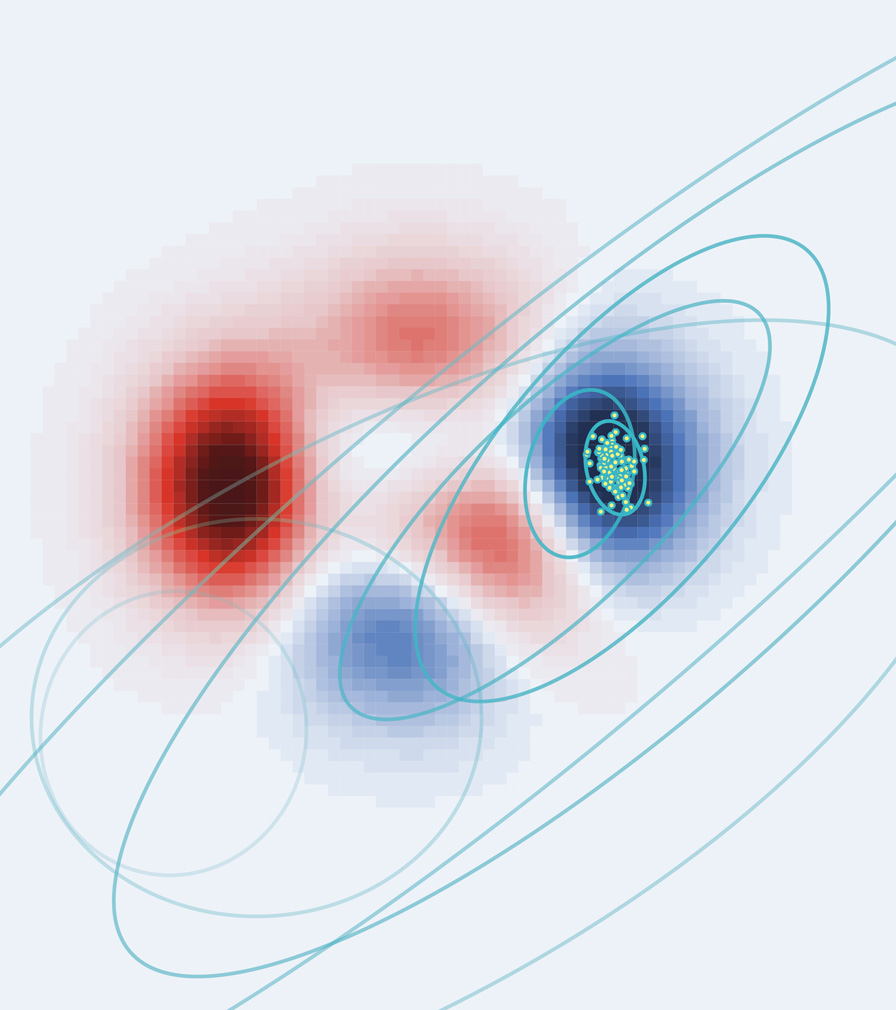
\includegraphics[width=1.0\linewidth]{chap9/9_0}
	% 加星号(*)表示不加编号
	\caption*{ \label{fig:9_0}}
\end{figure}


我一生中发现的最伟大的生物力学发现之一并非源于实验室,也未借助任何特殊设备,仅仅依靠人体不可思议的适应性。
1968年,一位名叫迪克$\cdot$福斯贝里的21岁土木工程系学生公布了他的发现,并在奥运会上以向后跳过跳高横杆的方式震惊了体育界。
一位体育记者写道:“福斯贝里跳过横杆就像一个人被人从30层楼的窗户推下去一样。”
然而,正是这种看似笨拙的跳高方式,让他创造了2.24米的奥运纪录,并最终获得金牌。


福斯贝里实际上是在高中时出于无奈才开始使用他的标志性技术。
他没能掌握当时的标准技术——“西部翻滚”,即跳高运动员面朝下越过横杆,仿佛用手臂和腿环抱横杆。
他还尝试了更古老的“剪刀”技术,即跳高运动员以近乎坐姿的姿势越过横杆,同时双腿像剪刀一样上下摆动。
但这种技术并不理想,因为跳高运动员必须将重心推到远高于横杆的高度。


在背越式跳高中,跳高运动员先向横杆一端跑去,然后向内弯曲身体,向中间跃过横杆,最后在最后一刻扭转身体,向后跃过横杆(图~\ref{fig:9_1})。
身体每次只滑过一个部位:
首先是头部和肩部,然后是躯干、臀部、膝盖,最后是双脚。
背越式跳高的一个优点是身体重心无需越过横杆。
在最高高度,臀部位于横杆上方时,背部拱起,头部和腿部悬在横杆下方,从而降低了重心。


\begin{figure}[!htb]
	\centering
	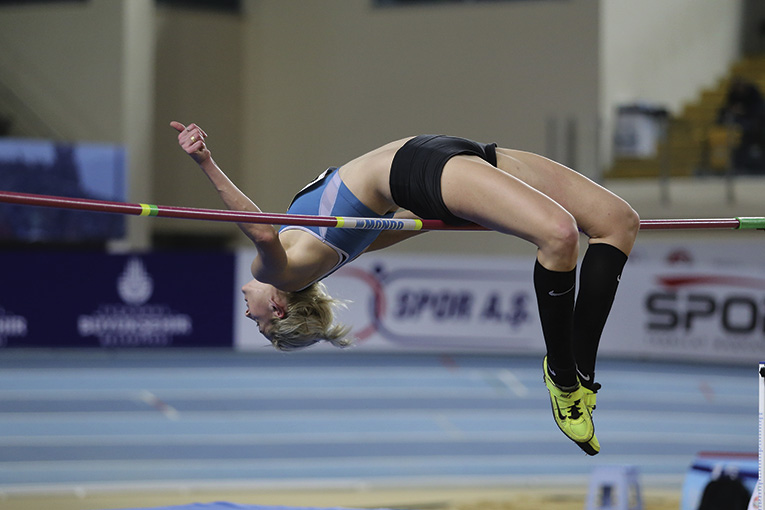
\includegraphics[width=1.0\linewidth]{chap9/9_1}
	\caption{“背越式跳高”技术。
		玛雅扬$\cdot$弗曼-沙哈夫的照片,摄影:埃夫伦$\cdot$卡林巴卡克。 \label{fig:9_1}}
\end{figure}


尽管福斯贝里在发明背越式跳高时并未接受过任何正规的生物力学训练,但我们现在已经赶上了他开创性的天才。
如今,教练们使用高速录像来指导跳高运动员脚部着地的位置、蹬地前蹲到多低等等。
他们想到了福斯贝里从未想过的改进。
起跳时抬起手臂可以增加垂直动能。
臀部越过横杆后收下巴有助于迫使臀部下沉,并根据牛顿第三运动定律,将双脚抬起并越过横杆。


自1980年以来,所有跳高世界纪录都是用背越式跳高创造的,其他所有技术都已从世界舞台上消失。
现在争论的焦点是哪种背越式跳高最好:
“速度背越式”还是“力量背越式”?


对我来说,福斯贝里跳马的故事教会了我几个宝贵的教训。
首先,我们永远不应该想当然地认为流行的做事方式就是唯一或最佳方式。
但一个不那么哲学、更偏向生物力学的信息是,我们的身体拥有关节骨骼和数百块肌肉,赋予我们完成任务的无限可能,无论是像端咖啡这样看似简单的动作,还是像跳两米高这样复杂的动作。
每一个动作都需要我们的大脑协调肌肉活动。
下巴的一个简单的动作就能对我们的双脚产生影响。


为了完成任何动作,我们的身体都会解决一个优化问题,试图用最小的努力获得最大的效果。
但有一个问题,无论是数学模型还是现实世界的运动员,都可能遇到难题:局部最优并不总是全局最优。
在背越式跳高之前的运动员们都认为他们找到了最佳技术。他们错了。
但他们无法仅仅通过对西方的滚翻技术进行小幅(“局部”)调整来提高标准。
他们需要一位愿意进行大规模(“全局”)调整的运动员工程师,来改变我们对跳高应该是什么样子的理解。


在本章中,我们将探讨 2 种使用数值优化计算肌肉力量的广泛场景。
第一种场景出现在我们希望\textit{估算产生可观测运动的肌肉力}时。
由于人体肌肉骨骼系统存在冗余,因此通常存在许多可能的解,我们将应用优化方法,找到符合某些标准的最佳肌肉力量集。
我们将这个问题称为肌肉冗余问题(也称为肌肉力量共享问题)。
第二种场景出现在研究肌肉协调性以\textit{优化特定任务的表现}时(例如跳高)。
在这种情况下,我们需要计算肌肉力以及完成任务的身体节段运动。
如果为优化器提供跳高比赛规则和足够逼真的肌肉骨骼系统模型,它就能发现背越式跳高(以及其他我们可能从未见过的技术)。
需要注意的是,使用优化方法估算肌肉力量不仅仅是为了计算上的便利:神经系统本身就是一种优化器。
让我们来深入了解一下细节。


\section{生物和数值优化器}

人们有意识地优化他们的日常生活。
我们会决定如何分配时间、金钱、注意力和其他有限的资源,以最大限度地平衡短期和长期的满足感,并在遵守法律和其他义务等约束的同时做到这一点。
令人惊讶的是,人类也会在潜意识中优化。
回想一下第二章,我们会自然地调整步行速度、步频和其他步态变量,以使我们的交通成本接近最低——当然,除非我们赶时间,在这种情况下我们会优先考虑速度而不是代谢成本。
在学习新任务和适应新情况时,我们也会在优化过程中,根据具体情况最大化准确性、效率、舒适度和其他性能指标的某种组合。
实验表明,我们会维持一个关于身体的“内部模型”,即潜意识地理解我们刺激肌肉的程度与由此产生的身体部位运动之间的关系。
当我们置身于新环境,例如国际空间站的微重力环境或机器人装置施加的人工力场时,我们最初会显得笨拙且效率低下,因为我们在规划和预测自身动作时使用的是一个不再精准的内部模型。
在探索新环境的过程中,我们会利用视觉和其他感官反馈来调整内部模型,提高协调性。
随着时间的推移,我们会适应新环境,并通过重新学习肌肉兴奋与运动表现之间的关系,重新获得熟练的技能。


数值优化算法使用类似的探索性或“猜测-检验”策略来寻找欠定问题的解。
我们将这些猜测称为候选解,每个候选解都为所有未知数或设计变量(例如肌肉冗余问题中的肌肉激励)提供了一个数值。
每个候选解的适用性通过评估目标函数或成本函数来确定,成本函数是量化特定设计变量值集合的可取性的表达式。
能够提供最佳目标函数值(视情况而定,最小值或最大值)的候选解被称为最优解,或者简称为优化问题的解(请注意,我们可以将我们的任务定义为始终寻求最小化目标函数;为了最大化像跳跃高度这样的量,我们只需最小化其负值即可)。
正如我们将看到的,目标函数的选择会对解以及计算它所需的工作量产生深远的影响。


最优解也会受到约束条件的影响。
在许多问题中,我们要求候选解满足某些表达式(等式或不等式),才能使其成为可行解或可接受的解。
例如,在肌肉冗余问题中,我们要求所有肌肉力均为拉伸力,并且它们产生的力矩之和等于所需的净关节力矩(例如,使用逆动力学算法计算)。
由于约束条件只能减少可行解的数量(即减小解空间的大小),因此,受约束优化问题的解的目标函数值并不比优化问题不受约束时更好。
添加约束会减少您的选择。
如果约束条件过多,解空间可能为空(问题可能没有可行解)。
根据研究问题的不同,可以将一个或多个严格约束转换为软约束,这些软约束以“惩罚”的形式添加到目标函数中。
惩罚项通常通过加权因子进行缩放,以便根据其相对重要性调整它们对目标函数的贡献。
通用优化问题可以表述如下:
%
\begin{proposition}[优化问题 1:找到产生所需关节力矩的踝跖屈肌力量] \label{pro:optim_1}
	
	\begin{equation}
		\begin{matrix}
			\text{最小化} & $ J(\underline{x}) $  & \text{调整设计变量 $ \underline{x} $ 以最小化目标函数 $ J(\underline{x}) $} \\
			% 
			$\text{受约束}$ & g_i(\underline{x}) \leq 0, i=1,...,n^i  & \text{同时满足 $ n $ 个不等式约束,} \\
			%
			& h_j (\underline{x}) = 0, j=1,...,n^j  &  \text{满足 $ n $ 个等式约束,} \\
			& \underline{x}^\text{lower} \leq \underline{x} \leq \underline{x}^\text{upper} & \text{并尊重设计变量的界限。}
		\end{matrix} \nonumber
	\end{equation}
	
\end{proposition}


我们潜意识地运用同样的原理来协调肌肉。
想象一下拿起桌上一支笔的动作。
你知道手所需的最终位置和方向,但你可以自由地(在一定范围内)选择手臂的最终姿势以及达到该姿势的路径。
正式地说,这个问题的每个候选解可能提出一组不同的肌肉激励,这些激励被定义为时间的参数化函数;这些参数将成为设计变量。
在所有候选解中,可行解是那些描述实现所需最终手部姿势的肌肉激励模式的解。
其他约束条件可能描述其他不可协商的要求,例如避开障碍物。
你大概会寻求在一定程度上最小化行程时间,但目标函数也可能包含一个有利于减少肌肉力量的项,用于完成这项非紧急任务。
解决此类问题的一种简单方法是评估所有可行解的目标函数,然后选择最佳候选解。
然而,正如您所料,所谓的“穷举搜索”(即考虑所有可能性)对于除最简单问题之外的所有问题都是低效且不切实际的。
数值优化器会尝试通过评估其认为必要的候选解数量来找到最有利的可行解(或至少是足以解决当前问题的可行解)。
许多优化器的区别仅在于它们如何根据已探索的候选解的适用性来选择新的候选解进行评估。


现在,我们将转向讨论解决肌肉冗余问题的策略。
为简单起见,我们将在某一时刻寻求解,假设所需的净关节矩已知,且对象静止不动。
我们有时将此类问题称为“静态”优化问题,因为其中忽略了一些与时间相关的因素。
在下一节中,我们将构建一个优化问题陈述,并通过观察求解一个简单的肌肉冗余问题,以建立对解空间的直觉。
在接下来的章节中,我们将讨论一些能够解决现实世界中遇到的非平凡优化问题的数值算法。



\section{通过检查解决静态优化问题}

我们首先关注图~\ref{fig:9_2}~所示的模型。假设我们希望产生 100 N$ \cdot $m 的踝关节跖屈净力矩。
应该激励哪些肌肉来产生这个力矩呢?有很多可行的方案。
例如,也许整个期望力矩都应该由比目鱼肌产生,或者最好是模型中的三个跖屈肌各自贡献一部分力矩。
背屈肌也可以产生力量,也可以由其中一块或两块背屈肌产生。
因此,该问题是欠定的:方程的数量少于未知数,我们需要更多信息来解决这个问题。
正式表述为,我们希望找到由每块肌肉 $ i $(我们的设计变量)产生的力 $ F_i $,使得踝关节跖屈总力矩为 100 N$ \cdot $m(等式约束),但前提是 $ F_i $ 为正,且对于任意 $ i = 1, ..., 5 $(界限)。


\begin{figure}[!htb]
	\centering
	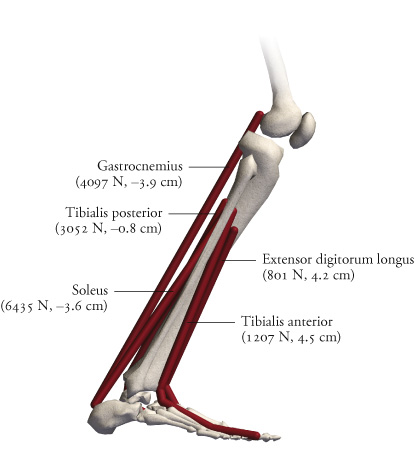
\includegraphics[width=0.7\linewidth]{chap9/9_2}
	\caption{小腿和足部的肌肉骨骼模型,包含关键的跖屈肌和背屈肌。
		测量的踝关节力矩可能由多种肌肉力量组合产生。
		括号中的值是瞬时最大力(假设速度为零且肌腱刚性)以及所示姿势对应的踝关节力臂。 \label{fig:9_2}}
\end{figure}


解决欠定问题的一种方法是修改问题,使方程的数量与未知数的数量相同。
在我们的示例中,为简单起见,我们假设背屈肌处于非活动状态,产生的力为 0。
% 腓肠肌:gastrocnemius 
% 比目鱼肌:soleus
% 胫骨后肌:tibialis posterior
这一假设将未知数的数量从 5 个减少到 3 个:腓肠肌(我们称之为 $ F_\text{GAS} $)、比目鱼肌($ F_\text{SOL} $)和胫骨后肌($ F_\text{TP} $)产生的力。
然而,我们仍然只有一个方程(指定期望净踝关节力矩的等式约束)。
我们可以假设每块跖屈肌都会产生相同的力,并引入 2 个附加方程,$ F_\text{SOL} = F_\text{GAS} $ 和 $ F_\text{TP} = F_\text{GAS} $。
这种策略可以得到一个可行的解,但通常不会产生生理上合理的结果。
相反,我们将定义一个目标函数 $ J(\underline{F}) $,它将解的有利性量化为肌肉力的函数,然后求解以下优化问题:
%
\begin{proposition}[优化问题 1:找到产生所需关节力矩的踝跖屈肌力量]

\begin{equation}
	\begin{aligned}
		\text{最小化} & J(\underline{F})  &  \text{目标函数中较小的值更受青睐} \\
		\text{受限于} & 0.039 F^\text{GAS} + 0.036 F^\text{SOL} + 0.008 F^\text{TP} & \text{肌肉必须产生所需的净踝关节力矩} \\
		& 0 \leq F^\text{GAS} \leq 4097 & \\
		& 0 \leq F^\text{SOL} \leq 6435 & \text{肌肉力量必须在生理范围内} \\
		& 0 \leq F^\text{TP} \leq 3052 &  \nonumber
	\end{aligned}
\end{equation}

\end{proposition}


例如,假设我们假设神经系统最小化每个时刻产生的总肌肉力,因此这就是瞬时肌肉力的总和:
%
\begin{equation}
	J ( \underline{F} ) 
		\triangleq
		F ^\text{GAS} + 
		F ^\text{SOL} + 
		F ^\text{TP} 
		= \sum_{i=1}^{3} F_i
	\label{eq:9_1}
\end{equation}

本例中的解是 $F^\text{GAS} = 2564$、$F^\text{SOL} = 0$ 和 $F^\text{TP} = 0$,因为腓肠肌具有最大的力臂,因此可以用最小的力量产生所需的踝关节跖屈力矩。
需要注意的是,在本模型中,腓肠肌能够产生完整的 100 N$\cdot$m 跖屈力矩(即 2564 N < 4097 N),实际上,当腓肠肌完全激活时,它可以在此姿势下产生约 160 N$\cdot$m 的力矩。
超过 160 N$\cdot$m 的踝关节力矩可以通过募集比目鱼肌(力臂第二大的肌肉)来产生,然后在比目鱼肌也达到最大力量后,再募集胫骨后肌(图~\ref{fig:9_3})。

\begin{figure}[!htb]
	\centering
	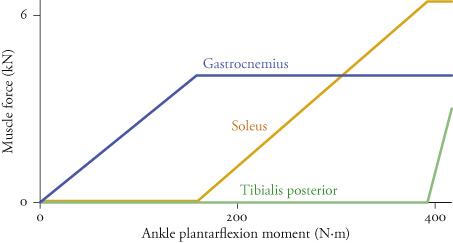
\includegraphics[width=0.75\linewidth]{chap9/9_3}
	\caption{图~\ref{fig:9_2}~中,假设肌肉协调策略最小化肌肉力量总和,则每块肌肉施加的力量会产生踝关节跖屈力矩。
		该目标函数(公式~\ref{eq:9_1})会导致不切实际的行为,即每块肌肉在下一块肌肉被调动之前就达到了其最大力量。 \label{fig:9_3}}
\end{figure}


虽然公式~\ref{eq:9_1}~中的目标函数可以很容易地求解优化问题,但请注意,当需要 100 N$\cdot$m 的跖屈力矩时,只会募集一块肌肉。
如果需要更大的力矩,则只有当第一块肌肉达到其最大产力能力时,我们才会募集第二块肌肉。
我们从实验中得知,肌肉实际上并非以这种逐步、非合作的方式募集。


不同的目标函数会导致不同的解决方案。
生物力学文献中提出了一些更切合实际的目标函数,但这些目标函数会导致无法通过检验解决的优化问题。
通常,我们必须使用计算机来解决生物力学中遇到的非线性、约束、高维问题。
在接下来的部分中,我们将讨论两大类优化算法:局部方法和全局方法。
然后,我们将继续解决一个更切合实际的肌肉力共享问题。



\section{解决静态优化问题的局部方法}

局部优化方法从一个初始猜测(候选解)开始,生成一系列新的猜测,每个猜测都与其前一个猜测相邻,并且通常具有更优的目标函数值。
当算法达到局部最优值时终止:该解在其紧邻域中被劣质解包围。
局部方法的一个典型示例是最速下降算法。
例如,如果我们求解一个二元最小化问题,目标函数 $J(x,y)$ 可以表示为一个曲面,其在点 $(x^*,y^*)$ 处高于 X-Y 平面的高度为 $J(x^*,y^*)$。
最速下降策略可以想象为将一颗弹珠放在目标函数曲面上,让它滚下山坡,直到落到盆底。
如图~\ref{fig:9_4}~所示,最终解取决于初始猜测,并且可能不是最佳解。
牛顿法与最速下降法类似,但它利用目标函数曲面的二阶导数(曲率)信息,更直接地逼近局部最小值——尽管计算这些额外信息的成本可能相当高。
内点法也很流行,它首先找到任意可行解(即可行域内部的解),然后在可行域内逐步寻找更优解。


\begin{figure}[!htb]
	\centering
	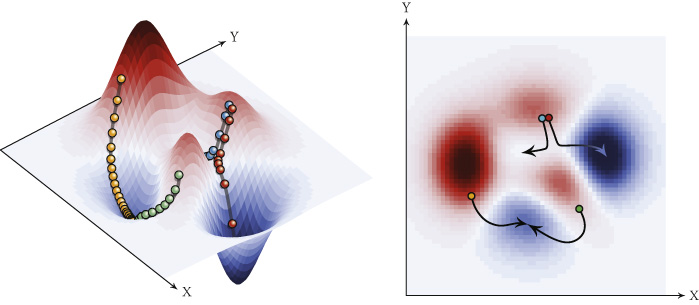
\includegraphics[width=1.0\linewidth]{chap9/9_4}
	\caption{两个变量目标函数的图形表示,其中曲面高度表示目标函数值 $J(x,y)$。
		最速下降算法从解空间中的某个点开始,沿着局部斜率最大的方向逐步下行,直到沿任何方向移动都能使 $J(x,y)$ 增加。
		最终解取决于初始猜测值,如此处所示的四条路径所示,并且可能并非全局最优。 \label{fig:9_4}}
\end{figure}


在图~\ref{fig:9_5}~中,我们展示了优化问题~\ref{pro:optim_1}(上文)的解决方案,该方案针对所有可能的踝关节跖屈力矩,同时最小化肌肉激活平方和,该平方和已被用作代谢能量消耗的替代品:


\begin{figure}[!htb]
	\centering
	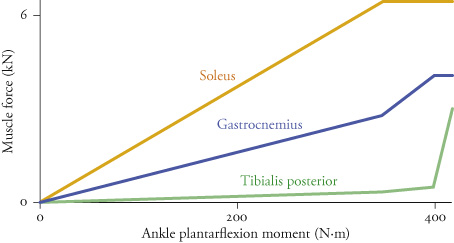
\includegraphics[width=1.0\linewidth]{chap9/9_5}
	\caption{图~\ref{fig:9_2}~中,假设肌肉协调策略最小化肌肉激活平方和,则每块肌肉为产生所有可能的踝关节跖屈力矩而施加的力。
		(公式~\ref{eq:9_2})得出的行为与实验观察结果一致,即即使产生微小的关节力矩,也会调动多块肌肉。 \label{fig:9_5}}
\end{figure}

\begin{equation}
	J ( \underline{F} ) 
		\triangleq 
		\sum_{i=1}^{3}
			( \frac{F_i}{F_i^\text{max}} )^2
		= 
		\sum_{i=1}^{3} a_i^2
	\label{eq:9_2}
\end{equation}


使用公式~\ref{eq:9_2}~计算出的肌肉活动比使用公式~\ref{eq:9_1}~所示的更简单的目标函数更接近人体实验中观察到的情况。
特别需要注意的是,在图~\ref{fig:9_5}~中,即使只需要较小的踝关节跖屈力矩,所有 3 块肌肉都会被募集,这与\textit{肌电图}的实验测量结果(图~\ref{fig:9_6})在定性上相似。


\begin{figure}[!htb]
	\centering
	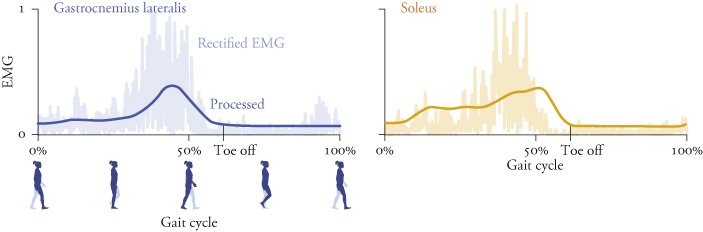
\includegraphics[width=1.0\linewidth]{chap9/9_6}
	\caption{行走时腓肠肌外侧肌(左)和比目鱼肌(右)的\textit{肌电图}信号。
		这两块肌肉都参与踝关节跖屈力矩的产生。数据来自 Bartlett 和 Kram (2008);Arnold 等人 (2013)。 \label{fig:9_6}}
\end{figure}


局部方法寻求其邻域内的最优解;然而,这样的局部最小值可能有很多。
例如,如图~\ref{fig:9_4}~所示,梯度下降算法找到的解取决于初始猜测。
我们或许可以尝试用不同的初始猜测运行该算法几次,但这仍然可能错过更好的(甚至可能好得多的)解。
记住迪克$\cdot$福斯贝里(Dick Fosbury)的名言。
此,尽管局部方法可能很快,但全局方法可能会产生更好的解。



\section{解决静态优化问题的全局方法}

全局优化方法通过考虑先前猜测值附近以外的候选解,避免“卡”入局部极小值。
遗传算法就是这样一种算法,其中候选解的种群通过模拟自然过程从一个阶段(一代)进化到下一个阶段。
这种优化策略背后的理念是更详细地探索解空间中已知有利的区域,同时也探索解空间中可能包含更优解的未探索区域。


遗传算法往往难以随问题规模的扩大而扩展,但其他进化算法在实践中表现良好。
例如,图~\ref{fig:9_7}~所示的协方差矩阵自适应进化策略 (CMA-ES) 对于存在许多局部最小值的高维问题表现非常出色。
在每一代中,CMA-ES 算法都会从一个分布中选择候选解,该分布的均值和协方差会根据前几代的偏好度进行更新。
随着时间的推移,该分布将逐渐趋近于一个解:均值将趋近于最优值,而分布则会收缩。
模拟退火算法采用了类似的思路;算法开始时会处于较高的“温度”,允许对解空间进行更具冒险精神的探索,然后逐渐“冷却”到更为保守的最速下降法。


\begin{figure}[!htb]
	\centering
	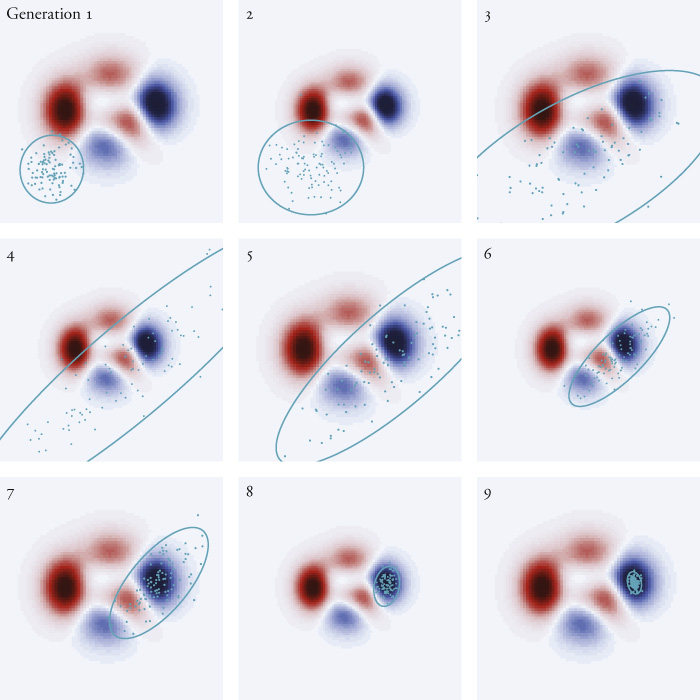
\includegraphics[width=1.0\linewidth]{chap9/9_7}
	\caption{协方差矩阵自适应进化策略 (CMA-ES) 等全局优化方法可以避免收敛到局部最小值。
		图中展示了 CMA-ES 算法的九代迭代过程,该算法最小化了图~\ref{fig:9_4}~所示的函数。
		每个青色点代表一个候选解;每个面板中的椭圆表示该代算法的种群分布。 \label{fig:9_7}}
\end{figure}


最佳优化器的选择取决于问题的性质。
例如,如果目标函数平滑且问题只有一个最小值,那么简单的局部搜索策略就足够了,因为它可以保证收敛到全局最小值。
另一方面,当存在许多局部最小值时,像 CMA-ES 这样的算法会更合适。
对于大型问题,使用可以并行运行的算法并定义标准来判断何时解足以解答特定的研究问题会更有利。



\section{行走和跑步时的肌肉力量}

有了这些优化方法,我们现在能够解决生物力学中最重要的问题之一:
确定负责产生行走和跑步等动作的肌肉力量。
这被称为肌肉冗余(或力量共享)问题。


当我们跑步时,在站立阶段的第一阶段,我们的肌肉会产生髋部伸展、膝部伸展和踝部跖屈的力矩。
假设我们希望计算在垂直地面反作用力达到峰值时产生的肌肉力(图~\ref{fig:9_8})。
使用图~\ref{fig:9_9}~中给出的下肢模型和数据,以及公式~\ref{eq:9_2}~中给出的目标函数来最小化肌肉激活平方和,我们可以将优化问题表达如下:


\begin{figure}[!htb]
	\centering
	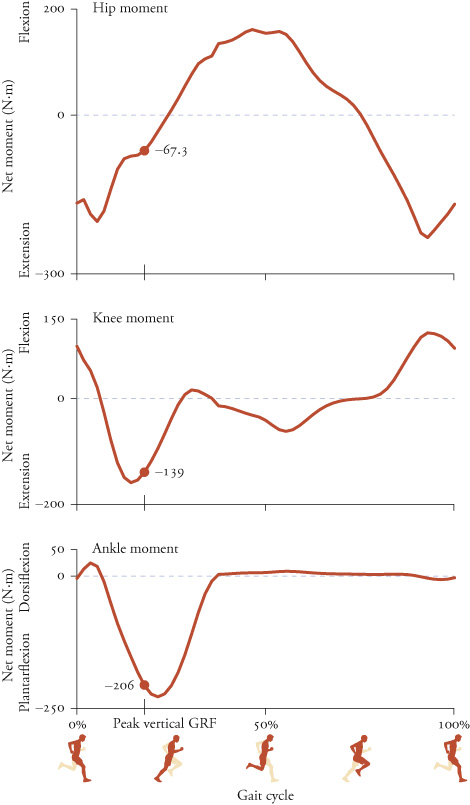
\includegraphics[width=0.7\linewidth]{chap9/9_8}
	\caption{一名受试者以 5 米/秒的速度奔跑时在矢状面上产生的净关节力矩。
		垂直线表示垂直地面反作用力 (GRF) 峰值出现的时间\cite{hamner2013muscle}。 \label{fig:9_8}}
\end{figure}


\begin{figure}[!htb]
	\centering
	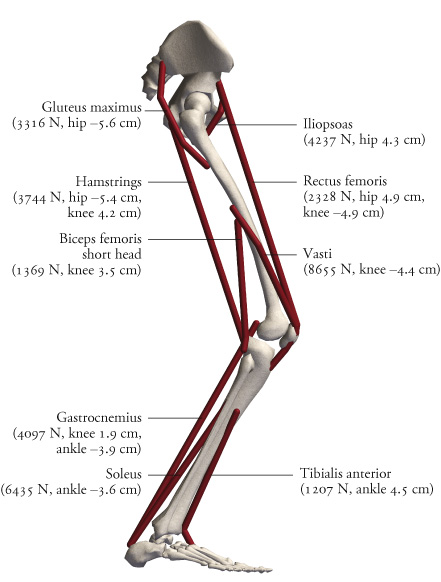
\includegraphics[width=0.7\linewidth]{chap9/9_9}
	\caption{一个简单的腿部肌肉骨骼模型可用于研究跑步站立阶段的肌肉协调性和关节负荷。
		参与产生矢状面运动的关键肌肉已被归类为九条代表性肌肉路径\cite{hamner2013muscle}。
		括号中的值是对应于所示姿势的瞬时最大力(假设速度为零且肌腱刚性)和力臂。 \label{fig:9_9}}
\end{figure}


\begin{proposition}[优化问题 2:找到跑步过程中垂直地面反作用力达到峰值时的肌肉激活情况]
	
	\begin{equation}
		\begin{aligned}
			\text{最小化} & J(\underline{a}) = \sum_{i=1}^{9} a_i ^2  \\
			\text{受限于} & \sum_{i=1}^{9} a_i ( r_i^\text{hip} F_i^\text{max} ) = -67.3 \\
			%
			& \sum_{i=1}^{9} a_i ( r_i^\text{knee} F_i^\text{max} ) = -139 \\
			& \sum_{i=1}^{9} a_i ( r_i^\text{ankle} F_i^\text{max} ) = -206 \\
			& 0 \leq a_i \leq 1 \; \text{for} \; i=1,...,9
			\nonumber
		\end{aligned}
	\end{equation}
	
\end{proposition}

该优化问题的解决方案是估计模型中每个肌肉在某一时间点产生的力量:

\begin{table}[htbp]
	\label{tab:9_1} \centering
	\begin{tabular}{cc} % l水平左居中,c水平居中
		\toprule
		肌肉或肌肉群 & 力, $F_i$牛  \\
		\midrule
		臀大肌 & 875  \\
		\midrule
		髂腰肌 & 0  \\
		\midrule
		腘绳肌 & 340  \\
		\midrule
		股直肌 & 0  \\
		\midrule
		股二头肌短头 & 0  \\
		\midrule
		股肌 & 4134  \\
		\midrule
		腓肠肌 & 1396  \\
		\midrule
		比目鱼肌 & 4167  \\
		\midrule
		胫骨前肌 & 0  \\
		\bottomrule
	\end{tabular}
\end{table}


通过在步态周期中均匀间隔的时刻重复此分析,我们可以估算出每块肌肉在行走和跑步过程中产生的力量。
图~\ref{fig:9_10}~和图~\ref{fig:9_11}~显示了行走状态下的肌肉力量及其产生的关节力矩;
图~\ref{fig:9_12}~和图~\ref{fig:9_13}~显示了跑步状态下的肌肉力量及其产生的关节力矩。
正如预期的那样,计算出的跑步状态下的肌肉力量高于行走状态下的肌肉力量。
还要注意的是,由于站立阶段较短,跑步状态下肌肉力量在步态周期中更早达到峰值,这也是我们预期的。


\begin{figure}[!htb]
	\centering
	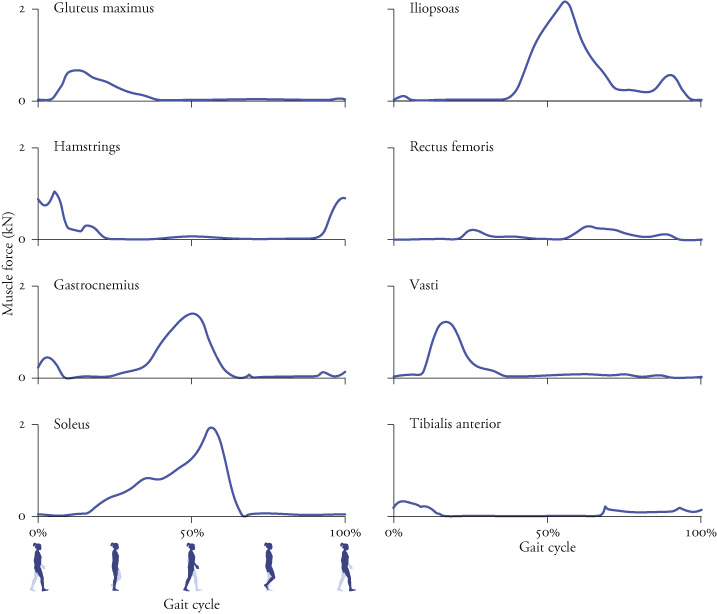
\includegraphics[width=1.0\linewidth]{chap9/9_10}
	\caption{使用 OpenSim 中的静态优化计算了一名受试者(男性,67.1 公斤)以自由选择的速度(1.67 米/秒)行走时的肌肉力量\cite{dembia2017simulating}。 \label{fig:9_10}}
\end{figure}


\begin{figure}[!htb]
	\centering
	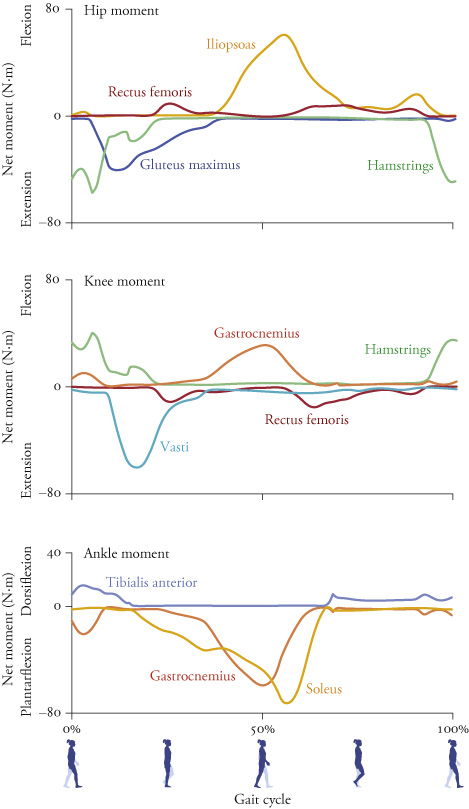
\includegraphics[width=0.8\linewidth]{chap9/9_11}
	\caption{如图~\ref{fig:9_10}~所示,以 1.67 m/s 的速度行走时,肌肉力量产生的矢状面关节力矩。 \label{fig:9_11}}
\end{figure}


\begin{figure}[!htb]
	\centering
	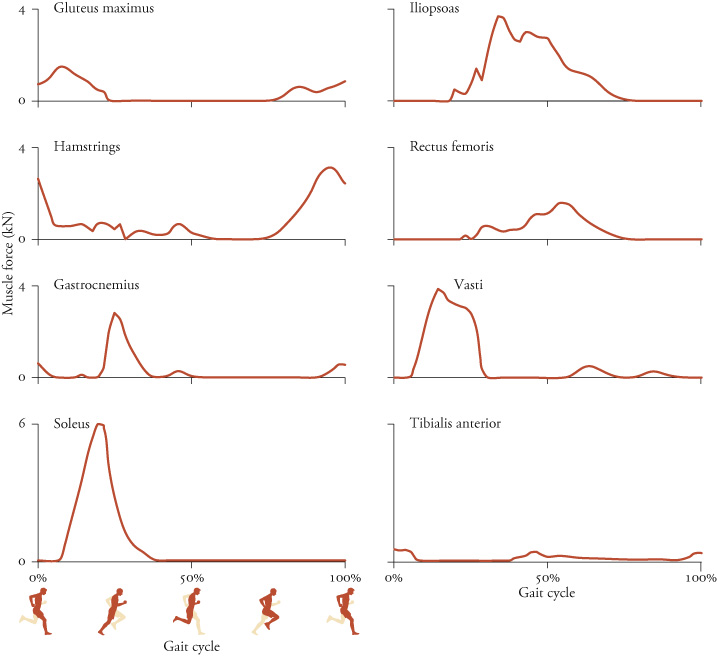
\includegraphics[width=1.0\linewidth]{chap9/9_12}
	\caption{一名受试者(男性,69.4 公斤)以 5 米/秒的速度奔跑时的肌肉力量,使用 OpenSim 中的静态优化计算得出\cite{hamner2013muscle}。 \label{fig:9_12}}
\end{figure}


\begin{figure}[!htb]
	\centering
	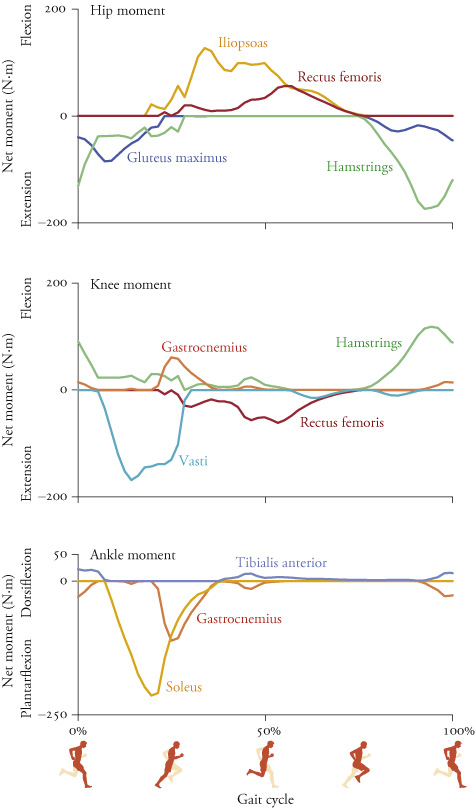
\includegraphics[width=0.8\linewidth]{chap9/9_13}
	\caption{以 5 m/s 的速度跑步时肌肉力量产生的矢状面关节力矩如图~\ref{fig:9_12}~所示。 \label{fig:9_13}}
\end{figure}


\section{估算关节负荷}

只有已知肌肉力量,才能估算关节负荷。
正如我们在第~\ref{chap:chap8}~章中提到的,区分通过逆动力学分析计算出的净关节反作用力和植入关节的传感器测量的“骨对骨”力至关重要。
只有当我们的肌肉像旋转马达一样施加纯关节扭矩时,我们在第~\ref{chap:chap8}~章中计算出的节段间力才会等于实际关节负荷。
当然,我们的肌肉并不直接产生扭矩,而是产生施加于骨骼的拉力。
这些力在关节中产生力矩以及压缩力和剪切力。
正如我们将看到的,肌肉力量对关节负荷的贡献可能很大。


为了演示肌肉力量如何影响关节负荷,我们考虑在5米/秒的速度下跑步时,垂直地面反作用力达到峰值的瞬间。
为简单起见,我们将使用图~\ref{fig:9_14}~所示的平面模型来计算踝关节的压缩力和剪切力。
在上一节中,我们使用了图~\ref{fig:9_9}~所示的下肢模型来估算腓肠肌和比目鱼肌在此瞬间产生的力。
但请注意,该模型中腓肠肌和比目鱼肌的路径并不位于垂直于踝关节轴线的平面内,因此在接下来的计算中,我们仅保留这些力在图~\ref{fig:9_14}~所示平面上作用的分量。
我们也将地面反作用力投射到这个平面上。
最后,我们假设足部在站立期处于静止状态,并按照第~\ref{chap:chap8}~章中的方法计算力$F_x$和$F_y$:


\begin{figure}[!htb]
	\centering
	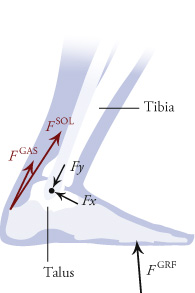
\includegraphics[width=0.3\linewidth]{chap9/9_14}
	\caption{平面模型用于估算以 5 米/秒的速度跑步时,垂直地面反作用力 (GRF) 达到峰值时的踝关节负荷。
		图中所示的力已投射到垂直于踝关节轴的平面上。 \label{fig:9_14}}
\end{figure}

\begin{equation}
	\begin{aligned}
		F_x & = F_x^\text{GAS} + 
				F_x^\text{SOL} + 
				F_x^\text{GRF} \\
			& = 44 \; \text{N} + 495\;\text{N} - 838 \; \text{N} \\
			& = -299 \;\text{N}
	\end{aligned}
	\label{eq:9_3}
\end{equation}


\begin{equation}
	\begin{aligned}
		F_y & = F_y^\text{GAS} + F_y^\text{SOL} + F_y^\text{GRF} \\
		& = 1357 \; \text{N} + 4088 \; \text{N} + 1379 \; \text{N} \\
		& = 6824 \; \text{N}
	\end{aligned}
	\label{eq:9_4}
\end{equation}


请注意,肌肉力量($F^\text{GAS}$ 和 $F^\text{SOL}$)对关节压缩力($F_y$)贡献巨大,约占总压缩力的 80\%。
本例中,跑步时的总压缩力超过 10 个体重,但在动态性较低的活动中也测量到了相当大的压缩负荷。
仪器化的人工关节记录到,行走时髋部峰值接触力约为 2.5 个体重,单腿站立不稳定时髋部峰值接触力超过 5 个体重。
即使在静止的单腿站立姿势下,由于肌肉产生的力量,髋部接触力也超过 2 个体重。
因此,如果我们想要评估关节内的力量,计算肌肉力量至关重要。


\section{动力学优化}

在前面的章节中,我们对待解决的底层优化问题做出了一些假设。
或许最重要的是,我们假设目标函数仅取决于瞬时量。
我们忽略了肌肉-肌腱动力学,并假设肌肉激活(以及由此产生的力量)仅取决于特定时刻所需的净关节力矩。
这类静态优化在计算上相对容易处理,但我们知道人类和动物都会预测未来。
例如,如果某个动作对后续有益,我们可能会在动作开始时投入能量,例如在投球前“收紧”,或在立定跳远前深蹲。
这些爆发性活动充分利用了我们肌肉和肌腱的动力学。
静态优化可能不足以完全理解投掷、跳跃和短跑等动作中的肌肉协调性,因为准确预测某一时间点的肌肉激活可能需要我们考虑整个动作。


我们在前几节中做出的第二个关键假设是,运动学和净关节矩是先验已知的。
例如,如果我们正在研究一个有运动捕捉数据的运动,我们可以使用逆运动学和逆动力学模拟来计算估算关节运动和矩。
然而,合适的实验数据可能无法获得,并且难以(或无法)收集,例如在研究高受伤率的活动或霸王龙的步态时。
此外,我们可能特别希望预测手术、植入物、假肢或外骨骼带来的未观察到的运动适应性,或者发现新的运动策略,以最大限度地提高运动表现或最大限度地减少关节负荷。
我们可以将动态优化用于这些任务。



在动态优化中,我们使用肌肉骨骼动力学模型来确定肌肉协调性及其相应的运动,从而优化运动任务的数学描述。
动态优化通常包括以下步骤:选择候选解,运行正向动态模拟,评估候选解的性能,并不断迭代直至满足某个停止标准(例如,达到目标函数值或已考虑预定数量的候选解;图~\ref{fig:9_15})。
设计变量可能包括肌肉骨骼参数,例如跟腱长度;可穿戴设备的参数,例如运动鞋的刚度;或每块​​肌肉随时间的活动情况。


\begin{figure}[!htb]
	\centering
	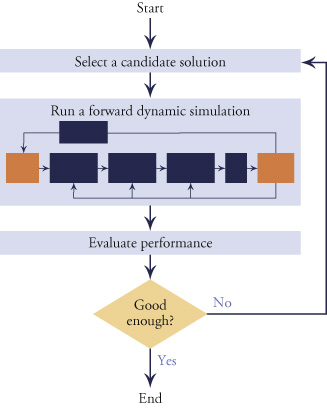
\includegraphics[width=0.55\linewidth]{chap9/9_15}
	\caption{动态优化的流程如下:
		选择候选解决方案,运行正向动态模拟,评估候选解决方案的性能,并不断迭代直至满足停止条件。
		候选解决方案可以由任何优化器选择,可以调整模型中的任何参数,并可以根据任何性能指标进行评估。 \label{fig:9_15}}
\end{figure}


例如,假设我们希望优化 100 米短跑过程中的肌肉协调性。
每个候选方案可能描述每块肌肉随时间的活动情况(例如,以参数化曲线或控制点序列的形式)。
我们将力求最大限度地缩短跑完 100 米所需的时间,并可能包含一些防止受伤的约束。
评估目标函数将涉及运行正向动态模拟(参见图~\ref{fig:1_12}),其中模型处于初始配置,在第一个时间点提出的激活应用于模型的肌肉,由此产生的肌肉力应用于骨骼,随后的加速度($\underline{F} = m \underline{a}$)在时间上进行数值积分,以确定模型在下一个时间点的配置,并重复该过程,直到跑步者到达终点线。
解决这个优化问题需要大量的计算资源。
为了使问题更易于处理,我们可以使用仅包含几个关键肌肉的平面模型,专注于固定速度的单个步态周期,或者设计神经控制器并优化相对较少的控制器参数,而不是在每个时间点激活每个肌肉。


目标函数和约束条件可以有多种形式,具体取决于所探讨的研究问题。
在上面的短跑示例中,我们只是试图最小化持续时间。
然而,对于像步行到公交车站或开门这样的任务,更合适的目标函数是将最小化持续时间与最小化总能量消耗结合起来,或许可以用反映活动紧急程度的权重来平衡这些项。
分析其他任务可能需要考虑安全性、舒适性、疲劳度和稳定性等因素的附加项。
需要注意的是,优化器非常“聪明”,它会利用优化问题中任何能够带来更优目标函数值的方面,而不管解决方案的主观性如何——所以要谨慎对待你的期望!我曾经定义过一个目标函数,用于最小化运输成本,而不设置最小行驶距离。
优化器明智地选择直接向前倒下,这消耗的能量很少,但这并不是我想要的。
定义优化问题可能是一个迭代过程,其中优化器返回的解用于识别从研究问题到目标函数和约束条件的转换过程中的错误。


与任何研究一样,验证优化结果至关重要。
如图~\ref{fig:9_6}~所示,计算出的肌肉活动时序可以与实验\textit{肌电图}时序进行比较。
实验运动学、地面反作用力、关节负荷(例如,来自器械关节置换)、间接量热法以及针对相同或类似活动的其他测量方法也可能有用。
动态优化的稳健且经过适当验证的结果可以深入了解运动和肌肉协调性。
例如,B. J. Fregly 利用优化方法发现了一种新的行走方式,可以减轻膝盖的负荷\cite{fregly2007design}。
他学会了以这种步态行走,因此,当他的孩子们去迪士尼乐园时,他能够跟上他们的步伐。


以背越式跳高为例,动态优化可能会发现,跳高运动员在离地时应该抬起双臂,以最大化其重心在起跳时的垂直速度。
同样,在起跳过程中,运动员应该尽可能长时间地与地面接触,以最大化地面反作用力的冲量。
这些洞见是通过背越式跳高首次亮相以来50年来运动员和教练员的经验积累而获得的。
相比之下,在下一节中,我们将描述一个通过计算机建模和数值优化更快地获得此类洞见的示例。



\text{立定跳远过程中的肌肉协调性}

矫形器、假肢和外骨骼等辅助设备有可能通过恢复受伤后的活动能力和提高运动表现来改善人类生活。
然而,我们尚未完全了解辅助设备在我们执行复杂任务时如何与肌肉协调相互作用。
我的学生卡迈克尔$\cdot$翁 (Carmichael Ong) 着手研究模拟辅助设备如何提高立定跳远的表现。
这项任务需要精确的肌肉协调,并且目标明确,因此非常适合进行优化。


Carmichael 使用了一个平面的五段模型(图~\ref{fig:9_16})。
位于踝关节、膝关节、髋关节和肩关节的生理扭矩执行器代表了穿过每个关节的所有肌肉的联合动作,并包含了生物肌肉中依赖于长度和速度的力产生能力。
每个扭矩执行器的活动用一个分段线性函数描述,其节点是动态优化问题中的设计变量。
该问题中的目标函数最大化跳跃距离。Carmichael 使用了一个平面的五段模型(图~\ref{fig:9_16})。
位于踝关节、膝关节、髋关节和肩关节的生理扭矩执行器代表了穿过每个关节的所有肌肉的联合动作,并包含了生物肌肉中依赖于长度和速度的力产生能力。
每个扭矩执行器的活动用一个分段线性函数描述,其节点是动态优化问题中的设计变量。
该问题中的目标函数最大化跳跃距离(通过最小化其负值),同时避免不良结果:
%
\begin{figure}[!htb]
	\centering
	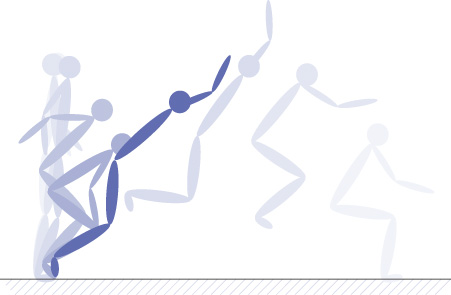
\includegraphics[width=0.8\linewidth]{chap9/9_16}
	\caption{一个包含五个段和七个自由度的平面模型,用于研究立定跳远过程中的肌肉协调性。
		采用动态优化方法预测踝关节、膝关节、髋关节和肩关节肌肉的协调性,以最大化跳跃距离\cite{ong2015simulation}。 \label{fig:9_16}}
\end{figure}


\begin{equation}
	\begin{bmatrix}
		\text{最小化} & J= & -d & \text{奖励更长的距离} \\
		& & + w_1 (J_\text{fall}) & \text{在着地时惩罚下降} \\
		& & + w_2 (J_\text{injury}) & \text{不鼓励使用韧带} \\
		& & + w_3 (J_\text{slip}) & \text{起跳时惩罚滑行} \\
		& & + w_4 (J_\text{time}) & \text{奖励反向运动}
	\end{bmatrix}
	\label{eq:9_5}
\end{equation}

公式~\ref{fig:9_5}~中的权重 $w_i$ 的选择是为了反映各项的相对重要性,并适当平衡长度、扭矩、力和时间的单位。
确定目标函数中的适当权重通常是一个迭代过程,需要手动调整或使用其他优化器(有时称为“元优化”)。


在本研究中,Carmichael 首先使用 CMA-ES 算法在无人协助的情况下优化模型的跳跃距离。
初始优化问题生成了立定跳远模型,该模型捕捉了人类跳跃的显著运动学和动力学特征,包括反向运动、起跳运动学、地面反作用力和关节力矩。
随后,他在臀部、膝盖和脚踝处放置了无质量旋转弹簧,增强了模型的可操作性(图~\ref{fig:9_17})。
当然,这样的装置并不存在,但模拟使我们能够以任何我们想要的方式调整施加的扭矩,这有助于我们了解它们如何影响运动表现。


\begin{figure}[!htb]
	\centering
	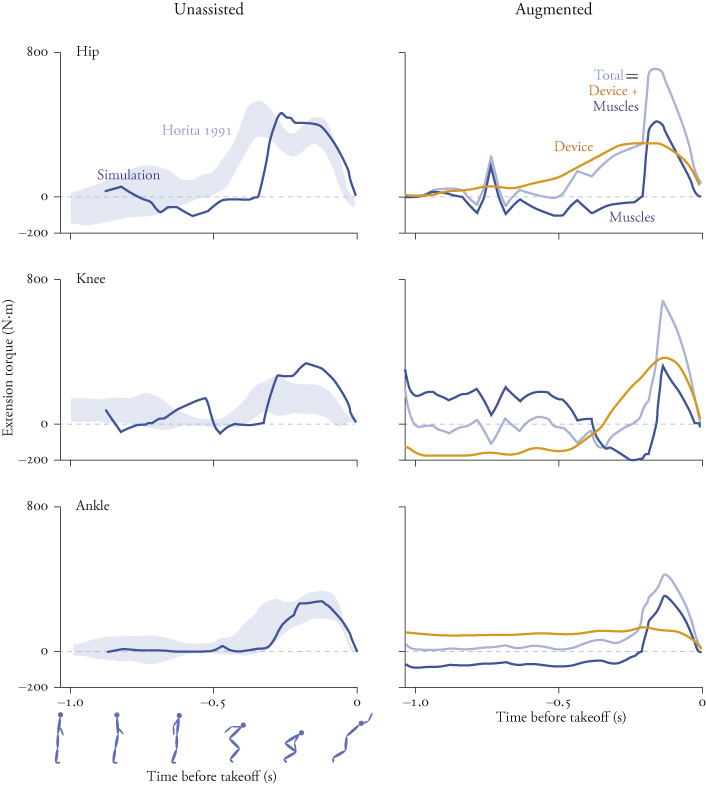
\includegraphics[width=1.0\linewidth]{chap9/9_17}
	\caption{立定跳远运动员在无辅助(左)和辅助(右)触地阶段的关节扭矩,其最大限度提升运动表现\cite{horita1991body}。 \label{fig:9_17}}
\end{figure}


在增强场景中,Carmichael 同时优化了每个弹簧的刚度和平衡位置以及其他设计变量。
优化后的辅助装置将跳跃距离增加了1米多,从2.27米增加到3.32米。
令人兴奋的是,该算法能够协同优化装置参数和人体协调性,使两者的综合性能实现了最长的跳跃距离。
这项研究展示了动态优化如何洞察人体运动,并补充辅助装置设计的实验方法。
未来,类似的预测工具或可用于为个体患者定制手术、植入物、假体或辅助装置,或许有助于确定哪种治疗方法能够带来最佳疗效。






